\documentclass[xcolor=dvipsnames]{beamer}
\usepackage[T1]{fontenc}
\usepackage[latin1]{inputenc}

\usepackage{geometry}
\usepackage{xcolor}
\usepackage{sansmathaccent}
\usepackage{dsfont}
\pdfmapfile{+sansmathaccent.map}
\usepackage{graphicx}
\usepackage[dvipsnames]{xcolor}
\usepackage{tikz}
\usetikzlibrary{arrows}
\usepackage{mathrsfs}
\usepackage{bm}
\usepackage{float}
\usepackage{algorithm}
\usepackage{algpseudocode}
%%%%%%%%%%%%%%%%%%%%%%%%%%%%%%%%%%%%%%%%%%%%



%%%%%%%%%%%%%%%%%%%%%%%%%%%%%%%%%%%%%%%%%%%%




\title[]{Solving Imperfect-Recall Games: \\ New Representations and Algorithms} 
\author[]{\textbf{Giulia Romano}}
\date{20 December 2018} 
\logo{
\includegraphics[scale=0.2]{PolimiLogo.png}}
\usetheme{CambridgeUS}
\usecolortheme[named=Maroon]{structure}
\setbeamercovered{dynamic}


\DeclareMathOperator*{\argmin}{arg\,min}
\DeclareMathOperator*{\argmax}{arg\,max}
\DeclareMathOperator*{\I}{\mathcal{I}}
\DeclareMathOperator*{\pl}{\mathcal{P}}
\DeclareMathOperator*{\T}{\mathcal{T}}
\DeclareMathOperator*{\F}{\mathcal{F}}
\DeclareMathOperator*{\B}{\mathcal{B}}
\DeclareMathOperator*{\A}{\mathcal{A}}
\DeclareMathOperator*{\ag}{\textbf{a}}
\DeclareMathOperator*{\pg}{\textbf{p}}


\begin{document}
	
	
	\setbeamercolor{uppercol}{fg=Blue,bg=white}
	\setbeamercolor{lowercol}{fg=black,bg=white}
	
		%1
		\begin{frame}
			\maketitle 
		\end{frame}
	   %2
	   \begin{frame}
	   \centering
	   \huge \alert{Preliminaries}
       \end{frame}
		
	    %3
	\section{Preliminaries}
	\begin{frame}
	\frametitle{Example of Normal-Form Game: Rock-Paper-Scissors}
	
	%A game in normal (strategic) form describes a strategic interaction in which each agent chooses his plan of action once and for all, and these choices are made simultaneously. 
	
	\begin{itemize}
		%come togliere spaziatura tra gli items?
		\item $\mathcal{P}=\{1,2\}$ 
		\item $A=\{A_1,A_2\}$ with $A_1=\{R,P,S\}$, $A_2=\{R,P,S\}$ 
	\end{itemize}
	
	\begin{table}
		
		\begin{tabular}{|l|c|c|r|}
			\hline
			& $R$ & $P$ & $S$ \\
			\hline
			$R$ & 0,0 & -1,1 & 1,-1  \\
			\hline
			$P$ & 1,-1 & 0,0 & -1,1  \\
			\hline
			$S$ & -1,1 & 1,-1 & 0,0  \\
			\hline
		\end{tabular}
	\end{table}  
\end{frame}	

	%3
	\begin{frame}
	\frametitle{Extensive-Form Games}
	\vspace{-.7cm}
	
	%A game in normal (strategic) form describes a strategic interaction in which each agent chooses his plan of action once and for all, and these choices are made simultaneously. 
	%\begin{definition}
	%	The normal-form representation of a game consists of a triplet $\langle \pl , (A_{i}), (\succsim_{i})\rangle$ where:
	%	\begin{itemize}
	%		\item $\pl=\{1,2,\ldots,n\}$ is the set of players;
	%		\item for each player $i \in \pl$, $A_{i}=\{a_{i,1},a_{i,2},\ldots,a_{i,m}\}$ is the set of actions available to player $i$;
	%		\item for each player $i \in \pl$, $\succsim_{i}$ is the preference relation on $A=\times_{j\in \pl}A_{j}$ of player $i$.
	%	\end{itemize}
	%\end{definition}
	
	\begin{definition}
		The extensive-form representation of a perfect-information game is a tuple $\langle \mathcal{P},A,H,Z,P,\pi_c,u\rangle$, where: 
		\begin{itemize}
			%come togliere spaziatura tra gli items?
			\item $\mathcal{P}=\{1,2,...,n\}$ is the finite set of players
			\item $A=\{A_1,A_2,...,A_n\}$, where $A_i$
			 is a finite set of actions of player $i$
			\item $H$ is a finite set of histories (i.e., sequences of actions)
			\item $Z\subseteq H$ is the set of terminal histories
			\item P : $H\to \pl$ is the function returning the player acting at a given decision node
			\item $\pi_c$ is the fixed strategy of a chance player
			\item $u=\{u_1,u_2,...u_n\}$ is the set of utility functions in which $u_i$ : $Z\to \mathbb{R}$
		\end{itemize}
	\end{definition}
    \end{frame}

%%%%%%%%%%%%%%%%%%%%%%%%%%%%%%%%%%%%%%%%%%%%%%%%%%%%%%%

\begin{frame}
\frametitle{Types of Extensive-Form Games}
\begin{minipage}{0.3\textwidth}
	\centering
	\begin{tikzpicture}[overlay]
	\node at (0.1,0.74) {\alert {\small{PERFECT INFORMATION}}};
	\end{tikzpicture}
	\begin{figure}[h]
		\centering
		\begin{tikzpicture}[line cap=round,line join=round,>=triangle 45,x=1cm,y=1cm,scale=0.6]
		\clip(-7.3,-3) rectangle (-1.9,3.5);
		\draw [line width=0.8pt] (-4.5,2)-- (-6,0);
		\draw [line width=0.8pt] (-6,0)-- (-7,-2);
		\draw [line width=0.8pt] (-6,0)-- (-5,-2);
		\draw [line width=0.8pt] (-4,-2)-- (-3,0);
		\draw [line width=0.8pt] (-3,0)-- (-2,-2);
		\draw [line width=0.8pt] (-3,0)-- (-4.5,2);
		
		
		\begin{scriptsize}
		\node at (-4.5,3) {\alert {\normalsize {Perfect Recall}}};
		\draw [fill=black] (-4.5,2) circle (2.5pt);
		\draw[color=black] (-4.5,2.37) node {$2.1$};
		\draw [fill=black] (-6,0) circle (2.5pt);
		
		\draw[color=black] (-5.401055826311682,1.33) node {$l_1$};
		\draw [fill=black] (-7,-2) circle (2.5pt);
		\draw[color=black] (-7.0849490746293675,-2.4) node {$x$};
		\draw[color=black] (-6.667837903027739,-0.7) node {$L_1$};
		\draw [fill=black] (-5,-2) circle (2.5pt);
		\draw[color=black] (-5.014841778532396,-2.4) node {$y$};
		\draw[color=black] (-5.27,-0.7) node {$R_1$};
		\draw [fill=black] (-4,-2) circle (2.5pt);
		\draw[color=black] (-4.010685254306254,-2.4) node {$z$};
		\draw [fill=black] (-3,0) circle (2.5pt);
		\draw[color=black] (-3.6708168922604827,-0.7) node {$L_2$};
		\draw [fill=black] (-2,-2) circle (2.5pt);
		\draw[color=black] (-2.0332693296763114,-2.4) node {$w$};
		\draw[color=black] (-2.239,-0.7) node {$R_2$};
		\draw[color=black] (-3.51,1.33) node {$r_1$};
		\draw[color=black] (-6.5,0.1) node {$1.1$};
		\draw[color=black] (-2.5,0.1) node {$1.2$};
		
		\end{scriptsize}
		\end{tikzpicture} 
	\end{figure}
\end{minipage}
\hspace{.2cm}
\vline
\pause
\begin{minipage}{0.5\textwidth}
	\centering
	\begin{tikzpicture}[overlay]
	\node at (3.7,2.97) {\alert {\small {IMPERFECT INFORMATION}}};
	\end{tikzpicture}
	\begin{minipage}{0.3\textwidth}
		\begin{figure}[H]
			\centering
			\definecolor{yqyqyq}{rgb}{0.5019607843137255,0.5019607843137255,0.5019607843137255}
			\definecolor{green}{rgb}{0.2,0.6,0}
			\begin{tikzpicture}[line cap=round,line join=round,>=triangle 45,x=1cm,y=1cm,scale=0.6]
			\clip(-7.3,-3) rectangle (-1.9,4);
			\draw [line width=0.8pt] (-4.5,2)-- (-6,0);
			\draw [line width=0.8pt] (-6,0)-- (-7,-2);
			\draw [line width=0.8pt] (-6,0)-- (-5,-2);
			\draw [line width=0.8pt] (-4,-2)-- (-3,0);
			\draw [line width=0.8pt] (-3,0)-- (-2,-2);
			\draw [line width=0.8pt] (-3,0)-- (-4.5,2);
			
			
			\begin{scriptsize}
			\node at (-4.5,3) {\alert {\normalsize {Perfect Recall}}};
			\draw [fill=black] (-4.5,2) circle (2.5pt);
			\draw[color=black] (-4.5,2.37) node {$2.1$};
			\draw [fill=black] (-6,0) circle (2.5pt);
			\draw [line width=0.8pt,dash pattern=on 2pt off 2pt, color=black] (-6,0)-- (-3,0);
			\draw[color=black] (-5.401055826311682,1.33) node {$l_1$};
			\draw [fill=black] (-7,-2) circle (2.5pt);
			\draw[color=black] (-7.0849490746293675,-2.4) node {$x$};
			\draw[color=black] (-6.667837903027739,-0.7) node {$L_1$};
			\draw [fill=black] (-5,-2) circle (2.5pt);
			\draw[color=black] (-5.014841778532396,-2.4) node {$y$};
			\draw[color=black] (-5.27,-0.7) node {$R_1$};
			\draw [fill=black] (-4,-2) circle (2.5pt);
			\draw[color=black] (-4.010685254306254,-2.4) node {$z$};
			\draw [fill=black] (-3,0) circle (2.5pt);
			\draw[color=black] (-3.6708168922604827,-0.7) node {$L_1$};
			\draw [fill=black] (-2,-2) circle (2.5pt);
			\draw[color=black] (-2.0332693296763114,-2.4) node {$w$};
			\draw[color=black] (-2.239,-0.7) node {$R_1$};
			\draw[color=black] (-3.51,1.33) node {$r_1$};
			\draw[color=black] (-4.5,0.3) node {$1.1$};
			\end{scriptsize}
			\pause
			\draw [line width=0.8pt, color=green] (-6,-0.3)-- (-3,-0.3);
			\draw [line width=0.8pt, color=green] (-6,0.3)-- (-3,0.3);
			\draw [line width=0.8pt, color=green] (-6,-0.3)-- (-6,0.3);
			\draw [line width=0.8pt, color=green] (-3,0.3)-- (-3,-0.3);
			\end{tikzpicture} 
		\end{figure} 

	\end{minipage}
	\hspace{1.8cm}
	\pause
	\begin{minipage}{0.3\textwidth}
		\begin{center}
			\begin{figure}[H]
				\centering
				\definecolor{green}{rgb}{0.2,0.6,0}
				\begin{tikzpicture}[line cap=round,line join=round,>=triangle 45,x=1cm,y=1cm,scale=0.6]
				\clip(-7.3,-3) rectangle (-1.9,4);
				
				\draw [line width=0.8pt] (-4.5,2)-- (-6,0);
				\draw [line width=0.8pt] (-6,0)-- (-7,-2);
				\draw [line width=0.8pt] (-6,0)-- (-5,-2);
				\draw [line width=0.8pt] (-4,-2)-- (-3,0);
				\draw [line width=0.8pt] (-3,0)-- (-2,-2);
				\draw [line width=0.8pt] (-3,0)-- (-4.5,2);
				
				
				\begin{scriptsize}
				\node at (-4.5,3) {\alert {\normalsize {Imperfect Recall}}};
				\draw [fill=black] (-4.5,2) circle (2.5pt);
				\draw[color=black] (-4.5,2.37) node {$1.1$};
				\draw [fill=black] (-6,0) circle (2.5pt);
				\draw [line width=0.8pt,dash pattern=on 2pt off 2pt, color=black] (-6,0)-- (-3,0);
				\draw[color=black] (-5.401055826311682,1.33) node {$L_1$};
				\draw [fill=black] (-7,-2) circle (2.5pt);
				\draw[color=black] (-7.0849490746293675,-2.4) node {$x$};
				\draw[color=black] (-6.667837903027739,-0.7) node {$L_2$};
				\draw [fill=black] (-5,-2) circle (2.5pt);
				\draw[color=black] (-5.014841778532396,-2.4) node {$y$};
				\draw[color=black] (-5.27,-0.7) node {$R_2$};
				\draw [fill=black] (-4,-2) circle (2.5pt);
				\draw[color=black] (-4.010685254306254,-2.4) node {$z$};
				\draw [fill=black] (-3,0) circle (2.5pt);
				\draw[color=black] (-3.6708168922604827,-0.7) node {$L_2$};
				\draw [fill=black] (-2,-2) circle (2.5pt);
				\draw[color=black] (-2.0332693296763114,-2.4) node {$w$};
				\draw[color=black] (-2.239,-0.7) node {$R_2$}; 
				\draw[color=black] (-3.51,1.33) node {$R_1$}; 
				\draw[color=black] (-4.5,0.3) node {$1.2$};	
			    \pause
			    \draw [line width=0.8pt, color=green] (-6,-0.3)-- (-3,-0.3);
			    \draw [line width=0.8pt, color=green] (-6,0.3)-- (-3,0.3);
			    \draw [line width=0.8pt, color=green] (-6,-0.3)-- (-6,0.3);
			    \draw [line width=0.8pt, color=green] (-3,0.3)-- (-3,-0.3);
				\end{scriptsize} 
				\end{tikzpicture} 
			 
				
			\end{figure} 
		\end{center}
	\end{minipage}
\end{minipage}
\end{frame}



   

%%%%%%%%%%%%%%%%%%%%%%%%%%%%%%%%%%%%%%%%%%%%%%%%%%%%%%%%%%%%%%%%%

\begin{frame}
\frametitle{From Extensive Form to Normal Form and Vice Versa}
\centering
\begin{tikzpicture}[line cap=round,line join=round,>=triangle 45,x=1cm,y=1cm, scale=0.74, font=\scriptsize]
\clip(-9.7,-4) rectangle (11.253323542996537,5);
\draw [line width=0.8pt] (-7,3)-- (-8,1);
\draw [line width=0.8pt] (-7,3)-- (-6,1);
\draw [line width=0.8pt] (-8,1)-- (-7.5,-1);
\draw [line width=0.8pt] (-8,1)-- (-8.5,-1);
\draw [line width=0.8pt] (-6,1)-- (-6.5,-1);
\draw [line width=0.8pt] (-6,1)-- (-5.5,-1);
\draw [rotate around={-89.34581818154798:(-7.0192824825678635,0.6887611820520816)},line width=1.5pt] (-7.0192824825678635,0.6887611820520816) ellipse (3.069015310028455cm and 2.5625317225449353cm);
\draw [->,line width=2pt] (-0.5,0.5) -- (-3.5,0.5);
\draw [->,line width=2pt] (-3.5,1.5) -- (-0.5,1.5);
\draw [line width=0.8pt] (2,1)-- (5,1);
\draw [line width=0.8pt] (2,1.5)-- (5,1.5);
\draw [line width=0.8pt] (2,0.5)-- (5,0.5);
\draw [line width=0.8pt] (2,0)-- (5,0);
\draw [line width=0.8pt] (2,-0.5)-- (5,-0.5);
\draw [line width=0.8pt] (3,2)-- (2.994921292626007,-0.5);
\draw [line width=0.8pt] (4,2)-- (4,-0.5);
\draw [rotate around={89.83148348743036:(3.5055742718060916,0.6612477740554176)},line width=1.5pt] (3.5055742718060916,0.6612477740554176) ellipse (3.045985198156396cm and 2.7039942425318824cm);
\begin{scriptsize}
\draw [fill=black] (-7,3) circle (2.5pt);
\draw[color=black] (-7,3.3) node {$2.1$};
\draw [fill=black] (-8,1) circle (2.5pt);
\draw[color=black] (-8.3,1.3) node {$1.1$};
\draw[color=black] (-7.719310435215781,2.48) node {$l_1$};
\draw [fill=black] (-6,1) circle (2.5pt);
\draw[color=black] (-5.6,1.3) node {$1.2$};
\draw[color=black] (-6.288143346135545,2.48) node {$r_1$};
\draw [fill=black] (-7.5,-1) circle (2.5pt);
\draw[color=black] (-7.5259094772319655,-1.24) node {$y$};
\draw[color=black] (-7.545249573030347,0.4759962228902294) node {$R_1$};
\draw [fill=black] (-8.5,-1) circle (2.5pt);
\draw[color=black] (-8.531594458747808,-1.24) node {$x$};
\draw[color=black] (-8.531594458747808,0.4759962228902294) node {$L_1$};
\draw [fill=black] (-6.5,-1) circle (2.5pt);
\draw[color=black] (-6.539564591514505,-1.24) node {$z$};
\draw[color=black] (-6.520224495716124,0.4759962228902294) node {$L_2$};
\draw [fill=black] (-5.5,-1) circle (2.5pt);
\draw[color=black] (-5.553219705797046,-1.24) node {$w$};
\draw[color=black] (-5.533879609998664,0.49533631868861094) node {$R_2$};
\draw[color=black] (2.4,1.27) node {$L_1L_2$};
\draw[color=black] (4.5,1.27) node {$z$};
\draw[color=black] (3.5,1.78) node {$l_1$};
\draw[color=black] (3.5,1.27) node {$x$};
\draw[color=black] (3.5,0.78) node {$x$};
\draw[color=black] (3.5,0.25) node {$y$};
\draw[color=black] (3.5,-0.25) node {$y$};
\draw[color=black] (4.5,1.78) node {$r_1$};
\draw[color=black] (2.4,0.78) node {$L_1R_2$};
\draw[color=black] (4.5,0.78) node {$w$};
\draw[color=black] (2.4,0.25) node {$R_1L_2$};
\draw[color=black] (4.5,0.25) node {$z$};
\draw[color=black] (2.4,-0.25) node {$R_1R_2$};
\draw[color=black] (4.5,-0.25) node {$w$};
\end{scriptsize}
\end{tikzpicture}

\end{frame}



%%%%%%%%%%%%%%%%%%%%%%%%%%%%%%%%%%%%%%%%%%%%%%%%%%%%%%%%%%%%%%%%%%
%4
\begin{frame}
\frametitle{Behavioral Strategies (Agent-Form Strategies)}
\begin{center}
	\begin{minipage}[c]{.70\textwidth}
		\centering
		\begin{figure}[h]
			
			\begin{tikzpicture}[line cap=round,line join=round,>=triangle 45,x=1cm,y=1cm,scale=0.7]
			\clip(-5,-5) rectangle (7,1);
			\draw [line width=0.8pt] (2,-2)-- (0,-4);
			\draw [line width=0.8pt] (2,-2)-- (4,-4);
			\draw [line width=0.8pt] (0,0)-- (-2,-2);
			\draw [line width=0.8pt] (0,0)-- (2,-2);
			\begin{scriptsize}
			\draw [fill=black] (-2,-2) circle (2.5pt);
			\draw[color=black] (-2.047530063532792,-2.5) node {$x$};
			\draw [fill=black] (2,-2) circle (2.5pt);
			\draw [fill=black] (0,-4) circle (2.5pt);
			\draw[color=black] (-0.040662554624467454,-4.5) node {$y$};
			\draw[color=black] (0.9418663299452332,-2.55) node {$L_2$};
			\draw [fill=black] (4,-4) circle (2.5pt);
			\draw[color=black] (3.973072463192182,-4.5) node {$z$};
			\draw[color=black] (3.0532581882758665,-2.55) node {$R_2$};
			\draw[color=black] (2.4,-1.8) node {$1.2$};
			\draw [fill=black] (0,0) circle (2.5pt);
			\draw[color=black] (-0.94,-0.48) node {$L_1$};
			\draw[color=black] (0.94,-0.48) node {$R_1$};
			\draw[color=black] (0,0.37879052755668985) node {$1.1$};
			\end{scriptsize}
			\end{tikzpicture}
		\end{figure}
	\end{minipage}%
	%\hspace{10mm}%
	\\
	\begin{minipage}[c]{.40\textwidth}
		\centering
		\begin{equation*}
		\pi_{1.1}=
		\begin{cases}
		\frac{1}{2}&L_1\\
		\frac{1}{2}&R_1
		\end{cases}
		\end{equation*}
	\end{minipage}
	%\hspace{10mm}%
	\begin{minipage}[c]{.40\textwidth}
		\centering
		\begin{equation*}
		\pi_{1.2}=
		\begin{cases}
		\frac{1}{2}&L_2\\
		\frac{1}{2}&R_2
		\end{cases}
		\end{equation*}
	\end{minipage}
\end{center}


\end{frame}

%%%%%%%%%%%%%%%%%%%%%%%%%%%%%%%%%%%%%%%%%%%%%%%%%%%%%%%%%%%%%%%%%%%%%%%%
 %4
 \begin{frame}
 \frametitle{Normal-Form Strategies}

\begin{minipage}{0.5\textwidth}
\begin{figure}
\begin{tikzpicture}[line cap=round,line join=round,>=triangle 45,x=1cm,y=1cm,scale=0.6]
		\clip(-5,-5) rectangle (7,1);
		\draw [line width=0.8pt] (2,-2)-- (0,-4);
		\draw [line width=0.8pt] (2,-2)-- (4,-4);
		\draw [line width=0.8pt] (0,0)-- (-2,-2);
		\draw [line width=0.8pt] (0,0)-- (2,-2);
\begin{scriptsize}
	\draw [fill=black] (-2,-2) circle (2.5pt);
	\draw[color=black] (-2.047530063532792,-2.5) node {$x$};
	\draw [fill=black] (2,-2) circle (2.5pt);
	\draw [fill=black] (0,-4) circle (2.5pt);
	\draw[color=black] (-0.040662554624467454,-4.5) node {$y$};
	\draw[color=black] (0.9418663299452332,-2.55) node {$L_2$};
	\draw [fill=black] (4,-4) circle (2.5pt);
	\draw[color=black] (3.973072463192182,-4.5) node {$z$};
	\draw[color=black] (3.0532581882758665,-2.55) node {$R_2$};
	\draw[color=black] (2.4,-1.8) node {$1.2$};
	\draw [fill=black] (0,0) circle (2.5pt);
	\draw[color=black] (-0.94,-0.48) node {$L_1$};
	\draw[color=black] (0.94,-0.48) node {$R_1$};
	\draw[color=black] (0,0.37879052755668985) node {$1.1$};
\end{scriptsize}
\end{tikzpicture}
\end{figure}
\end{minipage}
%
\hspace{.5cm}
\begin{minipage}{0.35\textwidth}
	\begin{table}
		\begin{center} 
			\begin{tabular}{c|c}
				Normal-form & Outcome \\
				plans & \\
				\hline
				\hline
				$L_1\ast$ & $x$ \\
				\hline
				$R_1 L_2$ & $y$ \\
				\hline
				$R_1 R_2$ & $z$ \\
			\end{tabular}
		\end{center}
	\end{table}
\end{minipage}
%\centering
%$\underbrace{ L_1* \quad R_1L_2 \quad R_1R_2 }_{Normal-Form ~ Plans}$
\end{frame}


%%%%%%%%%%%%%%%%%%%%%%%%%%%%%%%%%%%%%%%%%%%%%%%%%%%%%%%%%%%%%%%



%%%%%%%%%%%%%%%%%%%%%%%%%%%%%%%%%%%%%%%%%%%%%%%%%%%%%%%%%%%%%%%%%%%%%%%% 
   
   
    %5
%    \begin{frame}
%    \frametitle{Choice of the Strategy Representation}
%    %Perfect-Recall and Imperfect-Recall games
%    %Quando usare behavioral strategies e quando normal-form.
%    \textbf{PERFECT-RECALL GAMES}
%    \begin{block}{Khun Theorem}
%  	Given an extensive-form game and player $i \in \pl$, every normal-form strategy has an equivalent behavioral strategy if and only if $i$ has perfect recall.
%    \end{block}
% \textbf{Mixed Strategies}: the size of their space is exponential \\
% \textbf{Behavioral Strategies}:  the size of their space is linear\\
% 
% \vspace{+.5cm}
% 
% \textbf{IMPERFECT-RECALL GAMES}\\
% \textcolor{Maroon}{Khun Theorem} is not valid \\
%\textbf{Mixed Strategies}: are more expressive \\
%\textbf{Behavioral Strategies}: can cause a loss that is linearly large in the size of the game.
%    \end{frame}

\begin{frame}
\frametitle{Relationship between Strategies Representations}
\begin{block}{Khun Theorem}
	Given an extensive-form game and player $i \in \pl$, every normal-form strategy has an equivalent behavioral strategy if and only if $i$ has perfect recall.
\end{block}
\pause
\begin{itemize}
	\item \textbf{PERFECT-RECALL GAMES}
		\begin{itemize}
			\item \textbf{Khun Theorem} holds
			\item \textbf{Mixed Strategies}: the size of their space is exponential 
			\item \alert{\textbf{Behavioral Strategies}}:  the size of their space is linear
		\end{itemize}
	\pause
	\item \textbf{IMPERFECT-RECALL GAMES}
		\begin{itemize}
			\item \textbf{Khun Theorem} is not valid 
			\item \alert{\textbf{Mixed Strategies}}: more expressive 
			\item \textbf{\textcolor{blue}{Behavioral Strategies}}: can cause a loss that is linearly large in the size of the game. A Nash Equilibrium may not exist
		\end{itemize}
\end{itemize}
\end{frame}


\section{Original Contributions}

\begin{frame}
\centering
\huge \alert{Original Contributions}
\end{frame}

\begin{frame}
\frametitle{Summary of Results}
\begin{itemize}
	\item \textbf{BETTER REPRESENTATION}
	\begin{itemize}
		\item Imperfect-Recall Game $\leftrightarrow$ Team Perfect-Recall Game 
		\item Inflation
		\item Complexity of \textsf{MIN-P}
		\item ILP for minimizing the number of personalities
	\end{itemize}
	\pause
	\item \textbf{ALGORITHMS}
	\begin{itemize}
		    \item Polynomial-time algorithm for finding coarsest outer perfect-recall refinement
		    \item Column generation approach to compute mixed-strategy Nash Equilibrium in imperfect-recall game
			\item New best-response oracle that employs a pruning technique and uses information from the coarsest perfect-recall refinement 
	\end{itemize}
\end{itemize}
\end{frame}

\begin{frame}
\frametitle{Summary of Results}
\begin{itemize}
	\item \textbf{BETTER REPRESENTATION}
	\begin{itemize}
		\item \alert {Imperfect-Recall Game $\leftrightarrow$ Team Perfect-Recall Game }
		\item \alert {Inflation}
		\item \alert {Complexity of \textsf{MIN-P}}
		\item \alert {ILP for minimizing the number of personalities}
	\end{itemize}
	\item \textbf{ALGORITHMS}
	\begin{itemize}
		\item Polynomial-time algorithm for finding coarsest outer perfect-recall refinement
		\item Column generation approach to compute mixed-strategy Nash Equilibrium in imperfect-recall game
		\item New best-response oracle that employs a pruning technique and uses information from the coarsest perfect-recall refinement 
	\end{itemize}
\end{itemize}
\end{frame}

    %6

%%%%%%%%%%%%%%%%%%%%%%%%%%%%%%%%%%%%%%%%%%%%%%%%%%%%%%%%%%%%%%%%%%%%%%


    

    %8
%    \begin{frame}
%    \frametitle{The Notion of Personality}
%    %Def personalit�, valid assignement, gioco ausiliario.
%    %Esempio in cui mostro come un assegnamento di personalit� valido possa trasformare un giocatore imperfect recall in un team di perfect recall players.
%    \begin{definition}[Personality]\label{def:personality}
%    	Given a player $i\in\mathcal{P}$ with information partition $\mathcal{I}_i$, a personality $\tilde{\mathcal{I}}^k_i\subseteq\mathcal{I}_i$ is a subset of information sets such that an hypothetical player $j$ with $\mathcal{I}_j=\tilde{\mathcal{I}}^k_i$ would have perfect recall.
%    \end{definition}
%\pause
%\begin{definition}[Valid Assignment]
%	$\tilde{\mathcal{I}}_i=\{\tilde{\mathcal{I}}_i^1,\tilde{\mathcal{I}}_i^2,\ldots\}$ is a valid personality assignment for $i\in\mathcal{P}$ iff $\tilde{\mathcal{I}}_i$ is a partition of $\mathcal{I}_i$ and each element of $\tilde{\mathcal{I}}_i$ is a personality of player $i$.
%\end{definition} 
%\pause
%\begin{block}{Property}
%	In a two-player game $\Gamma$ where $i\in\mathcal{P}$ has imperfect recall and $-i\in\mathcal{P}$ has perfect recall, there is a bijection between the set of NE of $\Gamma$ and the set of TMECor of $\tilde{\Gamma}_i$.
%\end{block}
%    \end{frame}






\begin{frame}
\frametitle{The Notion of Personality}
Can we turn an imperfect-recall game into an equivalent perfect-recall one?
\pause
\begin{itemize}
	\item \alert{Team}: set of players sharing the same objectives
	\pause
	\item \alert{Personality}: given player $i\in\mathcal{P}$ with information partition $\mathcal{I}_i$, a personality $\tilde{\mathcal{I}}^k_i\subseteq\mathcal{I}_i$ is a subset of information sets such that an hypothetical player $j$ with $\mathcal{I}_j=\tilde{\mathcal{I}}^k_i$ would have perfect recall
\end{itemize}
\pause
\tikzstyle{block} = [rectangle, draw, fill=blue!20, 
text width=5em, text centered, rounded corners, minimum height=4em]
\tikzstyle{line} = [draw, -latex']

\vspace{.2cm}
\centering
\begin{tikzpicture}
\node[circle,draw=black, fill=white, inner sep=2pt,minimum size=5pt] (game) {$\Gamma$};

\node[block, right of=game, node distance=2.5cm, draw=black, fill=cyan!20, inner sep=2pt, minimum size=5pt] (realization) {Valid personality assignment};

\node[circle, right of=realization, node distance=2.5cm, draw=black, fill=yellow, inner sep=2pt,minimum size=5pt] (aux) {$\tilde{\Gamma}$};

\path [line] (game)--(realization);
\path [line] (realization)--(aux);

\node[block, below of=aux, node distance=2cm,draw=white, fill=white, inner sep=2pt,text width=9em] (th) {Auxiliary Perfect-Recall Team Game};
\path[line](th)--(aux);
\end{tikzpicture}
\pause
\vspace{-.5cm}
\begin{itemize}
\item \alert{Property}:\\
	Given $\Gamma$ where $i\in\mathcal{P}$ is imperfect recall, there is a bijection between the set of NE of $\Gamma$ and the set of TMECor of $\tilde{\Gamma}_i$
\end{itemize}

\end{frame}

   %8 
   \begin{frame}
   %\frametitle{Imperfect-Recall Completely-Inflated Game}
   \frametitle{Imperfect-Recall Game}
   $\I_1=\{1.1,1.2\}$ \quad $\I_2=\{2.1\}$
   
  \definecolor{yqyqyq}{rgb}{0.5019607843137255,0.5019607843137255,0.5019607843137255}
  \definecolor{ffffff}{rgb}{1,1,1}
  \begin{figure}
  	\centering
  	\begin{tikzpicture}[line cap=round,line join=round,>=triangle 45,x=1cm,y=1cm, scale=0.7]
  	\clip(-4.1721675137352925,-3.84352440307284) rectangle (11.860153241953327,4.8903195290852945);
  	\draw [line width=0.8pt] (3,4)-- (1.5,2);
  	\draw [line width=0.8pt] (3,4)-- (6,0);
  	\draw [line width=0.8pt] (1.5,2)-- (0,0);
  	\draw [line width=0.8pt] (1.5,2)-- (3,0);
  	\draw [line width=0.8pt] (0,0)-- (-1,-2);
  	\draw [line width=0.8pt] (0,0)-- (1,-2);
  	\draw [line width=0.8pt] (3,0)-- (2,-2);
  	\draw [line width=0.8pt] (3,0)-- (4,-2);
  	\draw [line width=0.8pt,dash pattern=on 2pt off 2pt, color=yqyqyq] (0,0)-- (6,0);
  	\draw [line width=0.8pt] (6,0)-- (5,-2);
  	\draw [line width=0.8pt] (6,0)-- (7,-2);
  	\begin{scriptsize}
  	\draw [fill=ffffff] (3,4) circle (2.5pt);
  	\draw[color=black] (2.9803397733245776,4.349015831340117) node {$2.1$};
  	\draw [fill=black] (1.5,2) circle (2.5pt);
  	\draw[color=black] (1,2.23245755251628) node {$1.1$};
  	\draw[color=black] (1.8369117376381354,3) node {$l_1$};
  	\draw [fill=black] (6,0) circle (2.5pt);
  	\draw[color=black] (4.184588449207107,3) node {$r_1$};
  	\draw [fill=black] (0,0) circle (2.5pt);
  	\draw[color=black] (0.5,1.3) node {$L_1$};
  	\draw [fill=black] (3,0) circle (2.5pt);
  	\draw[color=black] (3.6007103033246683,0.26186881016305197) node {$1.2$};
  	\draw[color=black] (2.45,1.3) node {$R_1$};
  	\draw [fill=black] (-1,-2) circle (2.5pt);
  	\draw[color=black] (-0.75,-0.77) node {$L_2$};
  	\draw [fill=black] (1,-2) circle (2.5pt);
  	\draw[color=black] (0.8,-0.77) node {$R_2$};
  	\draw [fill=black] (2,-2) circle (2.5pt);
  	\draw[color=black] (2.2,-0.77) node {$L_2$};
  	\draw [fill=black] (4,-2) circle (2.5pt);
  	\draw[color=black] (3.85,-0.77) node {$R_2$};
  	\draw [fill=black] (5,-2) circle (2.5pt);
  	\draw[color=black] (5.2,-0.77) node {$L_2$};
  	\draw [fill=black] (7,-2) circle (2.5pt);
  	\draw[color=black] (6.8,-0.77) node {$R_2$};
  	\end{scriptsize}
  	\end{tikzpicture}
  \end{figure}
   \end{frame}

%8 
\begin{frame}
\frametitle{Auxiliary Team Game}
\definecolor{green}{rgb}{0.2,0.6,0}
$\tilde{\I}^1_1=\{1.1\}$ \quad $\tilde{\I}^2_1=\{\textcolor{green}{3.1}\}$ \quad $\I_2=\{2.1\}$
\definecolor{yqyqyq}{rgb}{0.5019607843137255,0.5019607843137255,0.5019607843137255}
\definecolor{ffffff}{rgb}{1,1,1}
\begin{figure}
	\centering
	\begin{tikzpicture}[line cap=round,line join=round,>=triangle 45,x=1cm,y=1cm, scale=0.7]
	\clip(-4.1721675137352925,-3.84352440307284) rectangle (11.860153241953327,4.8903195290852945);
	\draw [line width=0.8pt] (3,4)-- (1.5,2);
	\draw [line width=0.8pt] (3,4)-- (6,0);
	\draw [line width=0.8pt] (1.5,2)-- (0,0);
	\draw [line width=0.8pt] (1.5,2)-- (3,0);
	\draw [line width=0.8pt] (0,0)-- (-1,-2);
	\draw [line width=0.8pt] (0,0)-- (1,-2);
	\draw [line width=0.8pt] (3,0)-- (2,-2);
	\draw [line width=0.8pt] (3,0)-- (4,-2);
	\draw [line width=0.8pt,dash pattern=on 2pt off 2pt, color=yqyqyq] (0,0)-- (6,0);
	\draw [line width=0.8pt] (6,0)-- (5,-2);
	\draw [line width=0.8pt] (6,0)-- (7,-2);
	\begin{scriptsize}
	\draw [fill=ffffff] (3,4) circle (2.5pt);
	\draw[color=black] (2.9803397733245776,4.349015831340117) node {$2.1$};
	\draw [fill=black] (1.5,2) circle (2.5pt);
	\draw[color=black] (1,2.23245755251628) node {$1.1$};
	\draw[color=black] (1.8369117376381354,3) node {$l_1$};
	\draw [fill=green] (6,0) circle (2.5pt);
	\draw[color=black] (4.184588449207107,3) node {$r_1$};
	\draw [fill=green] (0,0) circle (2.5pt);
	\draw[color=black] (0.5,1.3) node {$L_1$};
	\draw [fill=green] (3,0) circle (2.5pt);
	\draw[color=green] (3.6007103033246683,0.26186881016305197) node {$3.1$};
	\draw[color=black] (2.45,1.3) node {$R_1$};
	\draw [fill=black] (-1,-2) circle (2.5pt);
	\draw[color=black] (-0.75,-0.77) node {$L_2$};
	\draw [fill=black] (1,-2) circle (2.5pt);
	\draw[color=black] (0.8,-0.77) node {$R_2$};
	\draw [fill=black] (2,-2) circle (2.5pt);
	\draw[color=black] (2.2,-0.77) node {$L_2$};
	\draw [fill=black] (4,-2) circle (2.5pt);
	\draw[color=black] (3.85,-0.77) node {$R_2$};
	\draw [fill=black] (5,-2) circle (2.5pt);
	\draw[color=black] (5.2,-0.77) node {$L_2$};
	\draw [fill=black] (7,-2) circle (2.5pt);
	\draw[color=black] (6.8,-0.77) node {$R_2$};
	\end{scriptsize}
	\end{tikzpicture}
\end{figure}
\end{frame}

%\begin{frame}
%\frametitle{Complexity of MIN-P}
%We focus on the problem of computing the assignment $\tilde{\I}_i^\ast$ with the minimum possible cardinality. We call this problem \textsf{MIN-P}. \\
%The main hardness result states that \textsf{MIN-P} is \textsf{NP}-hard for the general class of imperfect-recall games. Then, we show that \textsf{MIN-P} remains hard on the subclass of completely inflated games.
%The main reduction is from \textsf{3-SAT}. 
%Given $\Gamma$ and $i\in\pl$, denote by \textsf{3-P} the problem of determining whether there exists $\tilde{\Gamma}_i$ such that $|\tilde{\I}_i|=3$.	\textsf{3-P} is \textsf{NP}-complete.
%
%Membership to \textsf{NP} follows from Lemma~\ref{lemma:check_valid}. To show that \textsf{3-P} is \textsf{NP}-hard, we provide a polynomial time reduction from \textsf{3-SAT} to \textsf{3-P}. Specifically, given a \textsf{3-SAT} instance $\phi$, we build an extensive-form game $\Gamma_\phi$ where a valid assignment with cardinality 3 is possible iff $\phi$ is satisfiable. $\Gamma_\phi$ is not robust with respect to inflation. 
%Therefore, after its description, we devise a structural transformation that can be repeatedly applied to $\Gamma_\phi$ to obtain a completely inflated tree ($\Gamma_\phi^\ast$). 
%%
%Since, $\Gamma_\phi$ and $\Gamma_\phi^\ast$ maintain the same properties with respect to the satisfiability of $\phi$, it is enough to show the correctness of the reduction over $\Gamma_\phi$.
%%
%\end{frame}


    %6
\begin{frame}
\frametitle{Inflation}

\textbf{Realization equivalence}:
Two strategies of player $i \in \pl$ are realization equivalent if, for every strategy of the opponents, they induce the same probability distribution over the outcomes of the game

%Definizione.
%Esempio in cui la applico a gioco imperfect recall.
%Risultato: algoritmo tempo polinomiale.
%dire che pu� essere usata come step di preprocessing
\pause
\begin{definition}[Immediate Inflation]\label{def:immediate_inflation}
	Let $\mathcal{I}_i$ and $\mathcal{I'}_i$ be two possible information partitions of player $i\in\mathcal{P}$. We say that $\mathcal{I'}_i$ is an immediate inflation of $\mathcal{I}_i$ iff there exist $I\in\mathcal{I}_i$ and $I_1,I_2\in\mathcal{I}'_i$ such that:
	\begin{itemize}%[nolistsep,itemsep=0mm]
		\item $I=I_1\cup I_2$ and $\mathcal{I}_i\setminus\{I\}=\mathcal{I'}_i\setminus\{I_1,I_2\}$;
		\item $\forall h_1\in I_1,h_2\in I_2$, there exists $\bar I\in\mathcal{I}_i\cap\mathcal{I'}_i$ such that $(\bar{I},a)\in X_i(h_1)$, $(\bar{I},b)\in X_i(h_2)$ and $a\ne b$.
	\end{itemize}
\end{definition}
\end{frame}


%%%%%%%%%%%%%%%%%%%%%%%%%%%%%%%%%%%%%%%%%%%%%%%%%%%%%%%%%%%%%%%%
\begin{frame}
\frametitle{Application of Inflation Operation}
\textbf{$\Sigma$-equivalence}: 
Two extensive-form games $\Gamma$ and $\Gamma'$ are $\Sigma$-equivalent if, $\forall i\in\pl$, $\forall\sigma_i\in\Sigma_i$ there exists a realization equivalent mixed strategy $\sigma_i'\in\Sigma_i'$, and vice versa

\vspace{.5cm}
\pause
\textbf{Example 1}: we obtain a perfect-recall game after applying inflation
\definecolor{yqyqyq}{rgb}{0.5019607843137255,0.5019607843137255,0.5019607843137255}
\begin{figure}
\centering
\begin{tikzpicture}[line cap=round,line join=round,>=triangle 45,x=1cm,y=1cm, scale=0.4]
\clip(-8,-2.2) rectangle (24,7);
\draw [line width=0.8pt] (-6,-2)-- (-4,2);
\draw [line width=0.8pt] (-4,2)-- (-2,-2);
\draw [line width=0.8pt] (2,2)-- (0,-2);
\draw [line width=0.8pt] (2,2)-- (4,-2);
\draw [line width=0.8pt,dash pattern=on 2pt off 2pt, color=yqyqyq] (-4,2)-- (2,2);
\draw [line width=0.8pt] (-1,6)-- (-4,2);
\draw [line width=0.8pt] (-1,6)-- (2,2);
\draw [->,line width=2pt] (5,2) -- (8,2);
\draw [line width=0.8pt] (10,-2)-- (12,2);
\draw [line width=0.8pt] (12,2)-- (14,-2);
\draw [line width=0.8pt] (16,-2)-- (18,2);
\draw [line width=0.8pt] (18,2)-- (20,-2);
\draw [line width=0.8pt] (15,6)-- (12,2);
\draw [line width=0.8pt] (15,6)-- (18,2);
\begin{scriptsize}
\draw [fill=black] (-6,-2) circle (4pt);

\draw [fill=black] (-4,2) circle (4pt);

\draw[color=black] (-5.5018031658684725,0.5) node {$L_2$};
\draw [fill=black] (-2,-2) circle (4pt);
\draw[color=black] (-2.6276882902218426,0.5) node {$R_2$};
\draw [fill=black] (2,2) circle (4pt);
\draw [fill=black] (0,-2) circle (4pt);
\draw[color=black] (0.6908773393907602,0.5) node {$L_2$};
\draw [fill=black] (4,-2) circle (4pt);
\draw[color=black] (3.35,0.5) node {$R_2$};
\draw[color=black] (-0.8795153246223465,2.7553986152460785) node {$1.2$};
\draw [fill=black] (-1,6) circle (4pt);
\draw[color=black] (-1.0,6.725825350675435) node {$1.1$};
\draw[color=black] (-2.7462084912794356,4.8) node {$L_1$};
\draw[color=black] (0.6908773393907602,4.8) node {$R_1$};


\draw [fill=black] (10,-2) circle (4pt);

\draw [fill=black] (12,2) circle (4pt);
\draw[color=black] (11.5,2.636878414188486) node {$1.2$};
\draw[color=black] (10.320643675320188,0.5) node {$L_2$};
\draw [fill=black] (14,-2) circle (4pt);
\draw[color=black] (13.461429003346401,0.5) node {$R_2$};
\draw [fill=black] (16,-2) circle (4pt);
\draw [fill=black] (18,2) circle (4pt);
\draw[color=black] (18.5,2.636878414188486) node {$1.3$};
\draw[color=black] (16.335543878993033,0.5) node {$L_3$};
\draw [fill=black] (20,-2) circle (4pt);
\draw[color=black] (19.476329207019244,0.5) node {$R_3$};
\draw [fill=black] (15,6) circle (4pt);
\draw[color=black] (15,6.63693519988224) node {$1.1$};
\draw[color=black] (13.16512850070242,4.8) node {$L_1$};
\draw[color=black] (16.957774934545395,4.8) node {$R_1$};
\end{scriptsize}
\end{tikzpicture}
\end{figure}

\end{frame}
%%%%%%%%%%%%%%%%%%%%%%%%%%%%%%%%%%%%%%%%%%%%%%%%%%%%%%%%%%%%%%%%%%%%%%

\begin{frame}
\frametitle{Completely-Inflated Tree}
\textbf{Example 2}: inflation cannot transform this imperfect-recall game in a perfect-recall one
\definecolor{yqyqyq}{rgb}{0.5019607843137255,0.5019607843137255,0.5019607843137255}
\definecolor{ffffff}{rgb}{1,1,1}
\begin{figure}
\centering
\begin{tikzpicture}[line cap=round,line join=round,>=triangle 45,x=1cm,y=1cm, scale=0.7]
\clip(-4.1721675137352925,-2.2) rectangle (9,4.5);
\draw [line width=0.8pt] (3,4)-- (1.5,2);
\draw [line width=0.8pt] (3,4)-- (6,0);
\draw [line width=0.8pt] (1.5,2)-- (0,0);
\draw [line width=0.8pt] (1.5,2)-- (3,0);
\draw [line width=0.8pt] (0,0)-- (-1,-2);
\draw [line width=0.8pt] (0,0)-- (1,-2);
\draw [line width=0.8pt] (3,0)-- (2,-2);
\draw [line width=0.8pt] (3,0)-- (4,-2);
\draw [line width=0.8pt,dash pattern=on 2pt off 2pt, color=yqyqyq] (0,0)-- (6,0);
\draw [line width=0.8pt] (6,0)-- (5,-2);
\draw [line width=0.8pt] (6,0)-- (7,-2);
\begin{scriptsize}
\draw [fill=ffffff] (3,4) circle (2.5pt);
\draw[color=black] (2.9803397733245776,4.349015831340117) node {$2.1$};
\draw [fill=black] (1.5,2) circle (2.5pt);
\draw[color=black] (1,2.23245755251628) node {$1.1$};
\draw[color=black] (1.8369117376381354,3) node {$l_1$};
\draw [fill=black] (6,0) circle (2.5pt);
\draw[color=black] (4.184588449207107,3) node {$r_1$};
\draw [fill=black] (0,0) circle (2.5pt);
\draw[color=black] (0.5,1.3) node {$L_1$};
\draw [fill=black] (3,0) circle (2.5pt);
\draw[color=black] (3.6007103033246683,0.26186881016305197) node {$1.2$};
\draw[color=black] (2.45,1.3) node {$R_1$};
\draw [fill=black] (-1,-2) circle (2.5pt);
\draw[color=black] (-0.75,-0.77) node {$L_2$};
\draw [fill=black] (1,-2) circle (2.5pt);
\draw[color=black] (0.8,-0.77) node {$R_2$};
\draw [fill=black] (2,-2) circle (2.5pt);
\draw[color=black] (2.2,-0.77) node {$L_2$};
\draw [fill=black] (4,-2) circle (2.5pt);
\draw[color=black] (3.85,-0.77) node {$R_2$};
\draw [fill=black] (5,-2) circle (2.5pt);
\draw[color=black] (5.2,-0.77) node {$L_2$};
\draw [fill=black] (7,-2) circle (2.5pt);
\draw[color=black] (6.8,-0.77) node {$R_2$};
\end{scriptsize}
\end{tikzpicture}
\end{figure}

\pause
We provide an algorithm that compute the \emph{complete inflation} of an extensive-form game in \textbf{polynomial time}
\end{frame}

%%%%%%%%%%%%%%%%%%%%%%%%%%%%%%%%%%%%%%%%%%%%%%

%7

%Abbiamo trovato un nuovo bound sull'ineffic. delle behavioral strategies che � robusto all'operazione di inflation.
% i primi livelli dell'albero usato nella proof: evidenzio i piani giocati con
%le miste e dico che invece con le behav. gioco uniformemente.
%altro motivo per scegliere le miste: le behav sono arbitrariamente peggio

\begin{frame}
\frametitle{New Bound on Behavioral Strategies' Inefficiency}
The loss incurred by a player when employing behavioral strategies in an \textbf{imperfect-recall game} may be linearly large in the size of the game
\begin{block}{Previous Inefficiency Bound}
Given a two-player game $\Gamma$ with player 1 having imperfect recall, take two strategy profiles $\sigma\in \times_{i\in\mathcal{P}}\Sigma_i $ and $\pi\in \times_{i\in\mathcal{P}}\Pi_i$ identifying two NE of the game. In the worst case, the ratio $u_1^\sigma/u_1^\pi$ is $|Z|/4$.
\end{block}

\pause
We extend the bound the class of \textbf{completely inflated games}

%This lower bound on behavioral strategies' ineciency is robust with respect to the ination operation and it strengthens the previously known bound of |Z|/4 by (Celli and Gatti, 2018). These bounds are asymptotically equivalent, except for logarithmic terms and constants.


%We provide a stronger inefficiency result.
%The key feature of the following construction is that it is robust with respect to the inflation operation, while the game instances used to obtain the previous bound can be significantly simplified through inflation.

\begin{block}{New Inefficiency Bound}
Given a two-player game $\Gamma$ with player 1 having imperfect recall, take two strategy profiles $\sigma\in \times_{i\in\mathcal{P}}\Sigma_i $ and $\pi\in \times_{i\in\mathcal{P}}\Pi_i$ identifying two NE of the game. In the worst case, the ratio $u_1^\sigma/u_1^\pi$ is $\Omega(|Z| (\frac{\log(\log(|Z|))}{\log(|Z|)})^3)$ even when the game is zero-sum, with binary payoffs.
\end{block}
\end{frame}





\begin{frame}
\frametitle{Complexity of MIN-P}
\begin{itemize}
	\item We call \textsf{MIN-P} the problem of finding a valid personality assignment with the minimum possible number of personalities %dire perch� � utile
	\item Sub-problem: \textsf{3-P}
	\item \textbf{Reduction from \textsf{3-SAT}}
\end{itemize}
\pause 

	\definecolor{ffffff}{rgb}{1,1,1}
	\definecolor{aqaqaq}{rgb}{0.6274509803921569,0.6274509803921569,0.6274509803921569}
	\definecolor{yqyqyq}{rgb}{0.5019607843137255,0.5019607843137255,0.5019607843137255}
	\definecolor{zzttqq}{rgb}{0.6,0.2,0}
		\centering
		\begin{tikzpicture}[line cap=round,line join=round,>=triangle 45,x=1cm,y=1cm,scale=0.15,font=\tiny]
		% scale=0.3,font=\tiny,rotate=90
		\clip(-31,-15.3) rectangle (34,23.5);
		\draw [line width=0.8pt] (2,22)-- (-7,18);
		\draw [line width=0.8pt] (2,22)-- (11,18);
		\draw [line width=0.8pt] (-7,18)-- (-12,14);
		\draw [line width=0.8pt] (-7,18)-- (-2,14);
		\draw [line width=0.8pt] (11,18)-- (4,14);
		\draw [line width=0.8pt] (11,18)-- (18,14);
		\draw [line width=0.8pt,dash pattern=on 2pt off 2pt, color=yqyqyq] (-7,18)-- (11,18);
		\draw [line width=0.8pt,dash pattern=on 2pt off 2pt, color=yqyqyq] (-12,14)-- (18,14);
		\draw [line width=0.8pt] (-12,14)-- (-17,10);
		\draw [line width=0.8pt] (-12,14)-- (-7,10);
		\draw [line width=0.8pt] (-2,14)-- (-4.2189582562205885,9.89179217090246);
		\draw [line width=0.8pt] (-2,14)-- (0,10);
		\draw [line width=0.8pt] (4,14)-- (2,10);
		\draw [line width=0.8pt] (4,14)-- (6,10);
		\draw [line width=0.8pt] (18,14)-- (12,10);
		\draw [line width=0.8pt] (18,14)-- (24,10);
		\draw [line width=0.8pt] (-17,10)-- (-18.977632576953663,6.022367423046338);
		\draw [line width=0.8pt] (-17,10)-- (-15,6);
		\draw [line width=0.8pt] (-7,10)-- (-8.977632576953663,6.022367423046338);
		\draw [line width=0.8pt] (-7,10)-- (-5,6);
		\draw [line width=0.8pt] (-18.977632576953663,6.022367423046338)-- (-22,2);
		\draw [line width=0.8pt] (-18.977632576953663,6.022367423046338)-- (-16,2);
		\draw [line width=0.8pt] (-8.977632576953663,6.022367423046338)-- (-12,2);
		\draw [line width=0.8pt] (-8.977632576953663,6.022367423046338)-- (-6,2);
		\draw [line width=0.8pt,dash pattern=on 2pt off 2pt, color=yqyqyq] (-22,2)-- (-6,2);
		\draw [line width=0.8pt,densely dotted] (-15,6)-- (-15.5,5);
		\draw [line width=0.8pt,densely dotted] (-15,6)-- (-14.5,5);
		\draw [line width=0.8pt,densely dotted] (-5,6)-- (-5.5,5);
		\draw [line width=0.8pt,densely dotted] (-5,6)-- (-4.5,5);
		\draw [line width=0.8pt] (-22,2)-- (-23.5,-2);
		\draw [line width=0.8pt] (-22,2)-- (-20.5,-2);
		\draw [line width=0.8pt] (-16,2)-- (-17.5,-2);
		\draw [line width=0.8pt] (-16,2)-- (-14.5,-2);
		\draw [line width=0.8pt] (-17.5,-2)-- (-19,-6);
		\draw [line width=0.8pt] (-17.5,-2)-- (-16,-6);
		\draw [line width=0.8pt] (-23.5,-2)-- (-25,-6);
		\draw [line width=0.8pt] (-23.5,-2)-- (-22,-6);
		\draw [line width=0.8pt] (-12,2)-- (-13.5,-2);
		\draw [line width=0.8pt] (-12,2)-- (-10.5,-2);
		\draw [line width=0.8pt] (-6,2)-- (-9,-2);
		\draw [line width=0.8pt] (-6,2)-- (-3,-2);
		\draw [line width=0.8pt] (-9,-2)-- (-10.5,-6);
		\draw [line width=0.8pt] (-9,-2)-- (-7.5,-6);
		\draw [line width=0.8pt] (-3,-2)-- (-4.5,-6);
		\draw [line width=0.8pt] (-3,-2)-- (-1.5,-6);
		\draw [line width=0.8pt] (-25,-6)-- (-26,-10);
		\draw [line width=0.8pt] (-25,-6)-- (-24,-10);
		\draw [line width=0.8pt] (-22,-6)-- (-23,-10);
		\draw [line width=0.8pt] (-22,-6)-- (-21,-10);
		\draw [line width=0.8pt] (-19,-6)-- (-20,-10);
		\draw [line width=0.8pt] (-19,-6)-- (-18,-10);
		\draw [line width=0.8pt] (-16,-6)-- (-17,-10);
		\draw [line width=0.8pt] (-16,-6)-- (-15,-10);
		\draw [line width=0.8pt] (-10.5,-6)-- (-11.5,-10);
		\draw [line width=0.8pt] (-10.5,-6)-- (-9.5,-10);
		\draw [line width=0.8pt] (-7.5,-6)-- (-8.5,-10);
		\draw [line width=0.8pt] (-7.5,-6)-- (-6.5,-10);
		\draw [line width=0.8pt] (-4.5,-6)-- (-5.5,-10);
		\draw [line width=0.8pt] (-4.5,-6)-- (-3.5,-10);
		\draw [line width=0.8pt] (-1.5,-6)-- (-2.5,-10);
		\draw [line width=0.8pt] (-1.5,-6)-- (-0.5,-10);
		\draw [line width=0.8pt,dash pattern=on 2pt off 2pt, color=yqyqyq] (2,10)-- (24,10);
		\draw [line width=0.8pt] (2,10)-- (1,6);
		\draw [line width=0.8pt] (2,10)-- (3,6);
		\draw [line width=0.8pt] (6,10)-- (5,6);
		\draw [line width=0.8pt] (6,10)-- (7,6);
		\draw [line width=0.8pt] (12,10)-- (11,6);
		\draw [line width=0.8pt] (12,10)-- (13,6);
		%\draw [line width=0.8pt] (24,10)-- (23,6);
		%\draw [line width=0.8pt] (24,10)-- (25,6);
		
		\draw [line width=0.8pt,densely dotted, color=aqaqaq] (-24,-4.4)-- (-23,-4.4);
		\draw [line width=0.8pt,densely dotted, color=aqaqaq] (-18,-4.4)-- (-17,-4.4);
		\draw [line width=0.8pt,densely dotted, color=aqaqaq] (-9.5,-4.4)-- (-8.497131029287853,-4.400164896934091);
		\draw [line width=0.8pt, densely dotted, color=aqaqaq] (-3.5,-4.4)-- (-2.5,-4.4);
		\draw [line width=0.8pt,densely dotted, color=aqaqaq] (-17.6,7.2)-- (-16.4,7.2);
		\draw [line width=0.8pt,densely dotted, color=aqaqaq] (-7.6,7.2)-- (-6.4,7.2);
		\draw [line width=0.8pt,densely dotted, color=aqaqaq] (1.6,7.2)-- (2.4,7.2);
		\draw [line width=0.8pt,densely dotted, color=aqaqaq] (5.6,7.2)-- (6.4,7.2);
		\draw [line width=0.8pt,densely dotted, color=aqaqaq] (11.6,7.2)-- (12.4,7.2);
		%\draw [line width=0.8pt,densely dotted, color=black] (23.6,7.2)-- (24.4,7.2);
		\draw [line width=0.8pt,dash pattern=on 2pt off 2pt, color=yqyqyq] (-17,10)-- (-7,10);
		
		\draw [shift={(-10.009477235991973,10.865742292277085)},line width=0.8pt,dash pattern=on 2pt off 2pt, color=yqyqyq]  plot[domain=3.914273764463971:5.5168699511464885,variable=\t]({1*6.938360585601049*cos(\t r)+0*6.938360585601049*sin(\t r)},{0*6.938360585601049*cos(\t r)+1*6.938360585601049*sin(\t r)});
		
		\draw [shift={(-14.009477235991973,10.865742292277085)},line width=0.8pt,dash pattern=on 2pt off 2pt, color=yqyqyq]  plot[domain=3.914273764463971:5.5168699511464885,variable=\t]({1*6.938360585601049*cos(\t r)+0*6.938360585601049*sin(\t r)},{0*6.938360585601049*cos(\t r)+1*6.938360585601049*sin(\t r)});
		\draw [shift={(-20.505857189101164,2.724785996638974)},line width=0.8pt,dash pattern=on 2pt off 2pt, color=yqyqyq]  plot[domain=4.147550998016063:5.278993934886491,variable=\t]({1*5.593611881967941*cos(\t r)+0*5.593611881967941*sin(\t r)},{0*5.593611881967941*cos(\t r)+1*5.593611881967941*sin(\t r)});
		\draw [shift={(-22.02838949796634,-0.5572829623136886)},line width=0.8pt,dash pattern=on 2pt off 2pt, color=yqyqyq]  plot[domain=4.2126379668602905:5.220141198173571,variable=\t]({1*6.201099719252835*cos(\t r)+0*6.201099719252835*sin(\t r)},{0*6.201099719252835*cos(\t r)+1*6.201099719252835*sin(\t r)});
		\draw [shift={(-19,-12)},line width=0.8pt,dash pattern=on 2pt off 2pt, color=yqyqyq]  plot[domain=1.1071487177940904:2.0344439357957027,variable=\t]({1*6.708203932499369*cos(\t r)+0*6.708203932499369*sin(\t r)},{0*6.708203932499369*cos(\t r)+1*6.708203932499369*sin(\t r)});
		\draw [line width=0.8pt,dash pattern=on 2pt off 2pt, color=yqyqyq] (-16,-6)-- (-11.321572541833424,-13.567162161905053);
		\draw [line width=0.8pt,dash pattern=on 2pt off 2pt, color=yqyqyq] (-25,-6)-- (-30,-6);
		\draw [shift={(-7.500314088155009,-1.3326677152038537)},line width=0.8pt,dash pattern=on 2pt off 2pt, color=yqyqyq]  plot[domain=4.141163995861399:5.283709206217189,variable=\t]({1*5.54816241889346*cos(\t r)+0*5.54816241889346*sin(\t r)},{0*5.54816241889346*cos(\t r)+1*5.54816241889346*sin(\t r)});
		\draw [shift={(-4.535830298917456,-12.014411366305403)},line width=0.8pt,dash pattern=on 2pt off 2pt, color=yqyqyq]  plot[domain=1.1033485004363943:2.0287031859764997,variable=\t]({1*6.737166295035983*cos(\t r)+0*6.737166295035983*sin(\t r)},{0*6.737166295035983*cos(\t r)+1*6.737166295035983*sin(\t r)});
		\draw [line width=0.8pt,dash pattern=on 2pt off 2pt, color=yqyqyq] (-1.5,-6)-- (3.046297265559931,-5.979095140375815);
		\draw [line width=0.8pt,dash pattern=on 2pt off 2pt, color=yqyqyq] (-4.5,-6)-- (-1.471258908390094,-14.02899479373211);
		
		\draw [shift={(3,9)},line width=0.8pt,dash pattern=on 2pt off 2pt, color=yqyqyq]  plot[domain=4.124386376837122:5.3003915839322575,variable=\t]({1*3.6055512754639896*cos(\t r)+0*3.6055512754639896*sin(\t r)},{0*3.6055512754639896*cos(\t r)+1*3.6055512754639896*sin(\t r)});
		\draw [shift={(8,11)},line width=0.8pt,dash pattern=on 2pt off 2pt, color=yqyqyq]  plot[domain=4.171969480114106:5.252808480655274,variable=\t]({1*5.8309518948453*cos(\t r)+0*5.8309518948453*sin(\t r)},{0*5.8309518948453*cos(\t r)+1*5.8309518948453*sin(\t r)});
		%\draw [shift={(17,19)},line width=0.8pt,dash pattern=on 2pt off 2pt, color=black]  plot[domain=4.279981204814152:5.144796755955228,variable=\t]({1*14.317821063276352*cos(\t r)+0*14.317821063276352*sin(\t r)},{0*14.317821063276352*cos(\t r)+1*14.317821063276352*sin(\t r)});
		\draw [shift={(5,3)},line width=0.8pt,dash pattern=on 2pt off 2pt, color=yqyqyq]  plot[domain=0.982793723247329:2.1587989303424644,variable=\t]({1*3.6055512754639896*cos(\t r)+0*3.6055512754639896*sin(\t r)},{0*3.6055512754639896*cos(\t r)+1*3.6055512754639896*sin(\t r)});
		\draw [shift={(10,0)},line width=0.8pt,dash pattern=on 2pt off 2pt, color=yqyqyq]  plot[domain=1.1071487177940904:2.0344439357957027,variable=\t]({1*6.708203932499369*cos(\t r)+0*6.708203932499369*sin(\t r)},{0*6.708203932499369*cos(\t r)+1*6.708203932499369*sin(\t r)});
		%\draw [shift={(19,-10)},line width=0.8pt,dash pattern=on 2pt off 2pt, color=black]  plot[domain=1.2120256565243244:1.929566997065469,variable=\t]({1*17.08800749063506*cos(\t r)+0*17.08800749063506*sin(\t r)},{0*17.08800749063506*cos(\t r)+1*17.08800749063506*sin(\t r)});
		\draw [line width=0.8pt,dash pattern=on 2pt off 2pt, color=yqyqyq] (-9,-2)-- (-3,-2);
		
		%%%%%%%%%%%%%%%%%%%%%%%%%%%%%%%%%%%%%%%%%%%%%%%%%%%%%%%%%
		\fill[line width=2pt,color=zzttqq,fill=zzttqq,fill opacity=0.10000000149011612] (20,6) -- (18,2) -- (22,2) -- cycle;
		\fill[line width=2pt,color=zzttqq,fill=zzttqq,fill opacity=0.10000000149011612] (28,6) -- (26,2) -- (30,2) -- cycle;
		
		
		\draw [line width=0.8pt] (24,10)-- (20,6);
		\draw [line width=0.8pt] (24,10)-- (28,6);
		\draw [line width=0.8pt] (1,6)-- (0.5,2);
		\draw [line width=0.8pt] (1,6)-- (1.5,2);
		\draw [line width=0.8pt] (5,6)-- (4.5,2);
		\draw [line width=0.8pt] (5,6)-- (5.5,2);
		\draw [line width=0.8pt] (11,6)-- (10.5,2);
		\draw [line width=0.8pt] (11,6)-- (11.5,2);
		
		\draw [line width=0.8pt,densely dotted, color=aqaqaq] (23.2,7.2)-- (24.8,7.2);
		\draw [line width=0.8pt] (3,6)-- (2.5,2);
		\draw [line width=0.8pt] (3,6)-- (3.5,2);
		\draw [line width=0.8pt] (7,6)-- (6.5,2);
		\draw [line width=0.8pt] (7,6)-- (7.5,2);
		\draw [line width=0.8pt] (13,6)-- (12.5,2);
		\draw [line width=0.8pt] (13,6)-- (13.5,2);
		\draw [line width=2pt,color=zzttqq] (20,6)-- (18,2);
		\draw [line width=2pt,color=zzttqq] (18,2)-- (22,2);
		\draw [line width=2pt,color=zzttqq] (22,2)-- (20,6);
		\draw [line width=2pt,color=zzttqq] (28,6)-- (26,2);
		\draw [line width=2pt,color=zzttqq] (26,2)-- (30,2);
		\draw [line width=2pt,color=zzttqq] (30,2)-- (28,6);
		\draw [line width=0.8pt,dash pattern=on 2pt off 2pt, color=yqyqyq] (27,4)-- (24.798470232164604,4.006958347218391);
		\draw [line width=0.8pt,dash pattern=on 2pt off 2pt, color=yqyqyq] (18.9885757213835,3.9771514427670036)-- (16.82073035275754,3.9830011704033534);
		\draw [line width=0.8pt,dash pattern=on 2pt off 2pt, color=yqyqyq] (20.59259191433479,4.814816171330422)-- (22.833981733331637,4.797545182114623);
		\draw [line width=0.8pt,dash pattern=on 2pt off 2pt, color=yqyqyq] (21.39141468988403,3.2171706202319403)-- (22.83764076260677,3.2339234181550314);
		\draw [line width=0.8pt,dash pattern=on 2pt off 2pt, color=yqyqyq] (28.596338092315296,4.80732381536941)-- (30.75920382436287,4.788551207273189);
		\draw [line width=0.8pt,dash pattern=on 2pt off 2pt, color=yqyqyq] (29.397106542549334,3.2057869149013323)-- (30.783249575068602,3.2015316606946813);
		\draw [shift={(20.430056471231097,-23.92544440423062)},line width=0.8pt,dash pattern=on 2pt off 2pt, color=yqyqyq]  plot[domain=1.323033629695652:1.8141607731322964,variable=\t]({1*30.86804606416558*cos(\t r)+0*30.86804606416558*sin(\t r)},{0*30.86804606416558*cos(\t r)+1*30.86804606416558*sin(\t r)});
		\draw [shift={(15.548687464814924,21.149066601163256)},line width=0.8pt,dash pattern=on 2pt off 2pt, color=yqyqyq]  plot[domain=4.420691931396036:4.998179441635736,variable=\t]({1*15.817230368779626*cos(\t r)+0*15.817230368779626*sin(\t r)},{0*15.817230368779626*cos(\t r)+1*15.817230368779626*sin(\t r)});
		%%%%%%%%%%%%%%%%%%%%%%%%%%%%%%%%%%%%%%%%%%%%%%%%%%%%%%%%%%%%
		\begin{scriptsize}
		\draw [fill=black] (2,22) circle (6pt);
		\draw [fill=black] (-7,18) circle (6pt);
		\draw [fill=black] (11,18) circle (6pt);
		\draw [fill=black] (-12,14) circle (6pt);
		\draw [fill=black] (-2,14) circle (6pt);
		\draw [fill=black] (4,14) circle (6pt);
		\draw [fill=black] (18,14) circle (6pt);
		\draw[color=black] (2.1,18.8) node {$F$};
		\draw[color=black] (2.1,14.8) node {$B$};
		\draw [fill=ffffff] (-17,10) circle (6pt);
		\draw [fill=ffffff] (-7,10) circle (6pt);
		\draw [fill=black] (-4.2189582562205885,9.89179217090246) circle (6pt);
		\draw [fill=black] (0,10) circle (6pt);
		\draw [fill=ffffff] (2,10) circle (6pt);
		\draw [fill=ffffff] (6,10) circle (6pt);
		\draw [fill=black] (12,10) circle (2.5pt);
		\draw[color=black] (9,10.63) node {$2.2$};
		\draw [fill=ffffff] (24,10) circle (6pt);
		\draw [fill=black] (-18.977632576953663,6.022367423046338) circle (6pt);
		\draw [fill=black] (-15,6) circle (6pt);
		\draw [fill=black] (-8.977632576953663,6.022367423046338) circle (6pt);
		\draw [fill=black] (-5,6) circle (6pt);
		\draw [fill=black] (-22,2) circle (6pt);
		\draw [fill=black] (-16,2) circle (6pt);
		\draw [fill=black] (-12,2) circle (6pt);
		\draw [fill=black] (-6,2) circle (6pt);
		\draw[color=black] (-13.98,2.6) node {$\bar{v}_1$};
		\draw [fill=ffffff] (-23.5,-2) circle (6pt);
		\draw [fill=black] (-20.5,-2) circle (6pt);
		\draw [fill=ffffff] (-17.5,-2) circle (6pt);
		\draw [fill=black] (-14.5,-2) circle (6pt);
		\draw [fill=black] (-19,-6) circle (6pt);
		\draw [fill=black] (-16,-6) circle (6pt);
		\draw [fill=black] (-25,-6) circle (6pt);
		\draw [fill=black] (-22,-6) circle (6pt);
		\draw [fill=black] (-13.5,-2) circle (6pt);
		\draw [fill=black] (-10.5,-2) circle (6pt);
		\draw [fill=ffffff] (-9,-2) circle (6pt);
		\draw [fill=ffffff] (-3,-2) circle (6pt);
		\draw [fill=black] (-10.5,-6) circle (6pt);
		\draw [fill=black] (-7.5,-6) circle (6pt);
		\draw [fill=black] (-4.5,-6) circle (6pt);
		\draw [fill=black] (-1.5,-6) circle (6pt);
		\draw [fill=black] (-26,-10) circle (6pt);
		\draw [fill=black] (-24,-10) circle (6pt);
		\draw [fill=black] (-23,-10) circle (6pt);
		\draw [fill=black] (-21,-10) circle (6pt);
		\draw [fill=black] (-20,-10) circle (6pt);
		\draw [fill=black] (-18,-10) circle (6pt);
		\draw [fill=black] (-17,-10) circle (6pt);
		\draw [fill=black] (-15,-10) circle (6pt);
		\draw [fill=black] (-11.5,-10) circle (6pt);
		\draw [fill=black] (-9.5,-10) circle (6pt);
		\draw [fill=black] (-8.5,-10) circle (6pt);
		\draw [fill=black] (-6.5,-10) circle (6pt);
		\draw [fill=black] (-5.5,-10) circle (6pt);
		\draw [fill=black] (-3.5,-10) circle (6pt);
		\draw [fill=black] (-2.5,-10) circle (6pt);
		\draw [fill=black] (-0.5,-10) circle (6pt);
		\draw [fill=black] (1,6) circle (6pt);
		\draw [fill=ffffff] (12,10) circle (6pt);
		\draw [fill=black] (3,6) circle (6pt);
		\draw [fill=black] (5,6) circle (6pt);
		\draw [fill=black] (7,6) circle (6pt);
		\draw [fill=black] (11,6) circle (6pt);
		\draw [fill=black] (13,6) circle (6pt);
		\draw[color=black] (-25,-4.5) node {$1$};
		\draw[color=black] (-22,-4.5) node {$\eta$};
		\draw[color=black] (-19,-4.5) node {$1$};
		\draw[color=black] (-16,-4.5) node {$\eta$};
		\draw[color=black] (-10.4,-4) node {$1$};
		\draw[color=black] (-7.6,-4) node {$\eta$};
		\draw[color=black] (-4.4,-4) node {$1$};
		\draw[color=black] (-1.6,-4) node {$\eta$};
		\draw[color=black] (-19,7.63) node {$1$};
		\draw[color=black] (-15,7.63) node {$m$};
		\draw[color=black] (-9,7.63) node {$1$};
		\draw[color=black] (-5,7.63) node {$m$};
		\draw[color=black] (0.8,7.67) node {$1$};
		\draw[color=black] (3.2,7.67) node {$\eta$};
		\draw[color=black] (4.8,7.67) node {$1$};
		\draw[color=black] (7.2,7.67) node {$\eta$};
		\draw[color=black] (10.8,7.67) node {$1$};
		\draw[color=black] (13.2,7.67) node {$\eta$};
		\draw[color=black] (20.8,7.67) node {$1$};
		\draw[color=black] (27.2,7.67) node {$\eta$};
		\draw[color=black] (-12,10.6) node {$2.1$};
		\draw[color=black] (-13.98,3.4) node {$v_1$};
		\draw[color=black] (-20.5,-3.6) node {$2.1.1$};
		\draw[color=black] (-13.234246492185454,-12.581216652397512) node {$\xi_1^{\eta}$};
		\draw[color=black] (-28.44229601676345,-5) node {$\xi_1^{1}$};
		\draw[color=black] (-6,-1.3) node {$2.1.2$};
		\draw[color=black] (2,-5) node {$\bar{\xi}_1^{\eta}$};
		\draw[color=black] (-0.91,-12.58) node {$\bar{\xi}_1^{1}$};
		\draw[color=black] (2.1,22.857318045195658) node {$T$};
		
		%%%%%%%%%%%%%%%%%%%%%%%%%%%%%%%%%%%%%%%%%%%%%%%%%
		
		\draw [fill=black] (0.5,2) circle (6pt);
		\draw [fill=black] (1.5,2) circle (6pt);
		\draw [fill=black] (4.5,2) circle (6pt);
		\draw [fill=black] (5.5,2) circle (6pt);
		\draw [fill=black] (10.5,2) circle (6pt);
		\draw [fill=black] (11.5,2) circle (6pt);
		\draw [fill=black] (2.5,2) circle (6pt);
		\draw [fill=black] (3.5,2) circle (6pt);
		\draw [fill=black] (6.5,2) circle (6pt);
		\draw [fill=black] (7.5,2) circle (6pt);
		\draw [fill=black] (12.5,2) circle (6pt);
		\draw [fill=black] (13.5,2) circle (6pt);
		\draw[color=zzttqq] (20.1,3.3) node {$C_1$};
		\draw[color=zzttqq] (28.1,3.3) node {$C_{\eta}$};
		\draw[color=black] (24.15,4.05) node {$\hat \xi_1^{\eta}$};
		\draw[color=black] (16.2,4.05) node {$\hat \xi_1^{1}$};
		\draw[color=black] (22.119916919694365,5.6) node {$\hat \xi_2^{1}$};
		\draw[color=black] (22.9,2.5) node {$\hat \xi_3^{1}$};
		\draw[color=black] (30.08683768415206,5.6) node {$\hat \xi_2^{\eta}$};
		\draw[color=black] (31.05,2.5) node {$\hat \xi_3^{\eta}$};
		%%%%%%%%%%%%%%%%%%%%%%%%%%%%%%%%%%%%%%%%%%%%%%%%%%%%%%%%%
		
		\end{scriptsize}
		\end{tikzpicture}

\end{frame}

\begin{frame}{Complexity of \textsf{MIN-P}}

\textsf{3-P} over $\Gamma_\phi$ is satisfiable  if and only if $\phi$ is satisfiable 
\pause

\begin{theorem}\label{th:hardness}
	\textsf{MIN-P} is \textsf{NP}-hard.
\end{theorem}
\pause

\begin{corollary}\label{th:hardness_2}
	\textsf{MIN-P} is \textsf{NP}-hard even for the class of completely inflated games.
\end{corollary}

%This shows that, despite the existence of a valid personality assignment is guaranteed, it is difficult to find an optimal personality allocation. Notice that, in order to reduce the number of required personalities, one could use inflation (in particular, Algorithm~\ref{alg:inflation}) as a preprocessing step before building an auxiliary team game. Now we show an example where an approximation algorithm by \citep{basilico2017} provides an arbitrarily better solution if applied to the game obtained minimizing the personalities rather than to the original game.

\pause
\begin{theorem}\label{th:apx}
	\textsf{MIN-P} is \textsf{APX}-hard, and no better approximation than $4/3$ is possible in polynomial time, unless $\textsf{P}=\textsf{NP}$.
\end{theorem}

%For $\Gamma_\phi$ game instances, there exists a polynomial time approximation algorithm with an approximation ratio bounded by $4/3$ (the optimal ratio being 1). Solving \textsf{MIN-P} over $\Gamma_\phi$s within every multiplicative factor lower than $4/3$ requires exponential time~(Theorem~\ref{th:hardness}). Therefore, \textsf{MIN-P} is \textsf{APX}-hard.

\end{frame}



    %8
    %\begin{frame}
    %\frametitle{Results}
    %MIN-P � NP-hard (anche per giochi completely inflated).\\
    %MIN-P is APX-hard, and no better approximation than $4/3$ is possible in polynomial time, unless $P=NP$.
    %\end{frame}

    %9
    \begin{frame}
    \frametitle{ILP for Minimizing the Number of Personalities}
    In this section we describe an ILP in order to find a valid minimum personality assignment
   	\begin{align*}
    \min_{w,P} & ~ \mathds{1}^{T}\textbf{w} & \\
    \textnormal{s.t. }& \mathds{1}^{T}P_{\cdot j} = 1 &\forall j\in \{1,...,|{\I}_{1}|\} \\
     & w_i \ge \frac{1}{|{\I}_{1}|}P_{i \cdot}\mathds{1} & \forall i \in \{1,...,|{\I}_{1}|\} \\
     & P_{i,j} + P_{i,k} - 1 \le M_{j,k}  \begin{split}\forall i \in \{1,...,|{\I}_{1}|\},\\\forall (j,k) \in \{1,...,|{\I}_{1}|\} \times \{1,...,|{\I}_{1}|\}\\\textnormal{s.t. } k>j\end{split}&\\
     & \textbf{w} \in \{0,1\}^{|{\I}_1|} &  \\
     & \textbf{P} \in \{0,1\}^{|{\I}_1| \times |{\I}_1|} & \\
    \end{align*}
    \end{frame}


 
%14
\begin{frame}
\frametitle{Conclusions}
\begin{itemize}
	\item The complete inflation of a game can be computed in polynomial time
	\item MIN-P is \textsf{NP}-hard, and even hard to approximate
	\item We provided an ILP for minimizing the number of personalities
	\item We presented an improved column generation approach for finding an optimal mixed-strategy Nash equilibrium in imperfect-recall games
	\begin{itemize}
		\item new best-response oracle that employs a pruning technique and uses information from the coarsest perfect-recall refinement 
	\end{itemize}
\end{itemize}
\end{frame}

    

    %14
    \begin{frame}
    \frametitle{Future Developments}
    \begin{itemize}
    	\item Evaluate, in a practical scenario, the impact of inflation in terms of \emph{split} information sets
    	%This operation may be effectively applied as a preprocessing step before looking for a valid personality assignment.
    	\item Our negative results on MIN-P suggest that it would be interesting to study algorithmic techniques for equilibrium computation in team games that are \emph{robust} with respect to the number of team members
    	\item Experimentally evaluate our best-response oracle against current known techniques for the problem
    \end{itemize}
    \end{frame}

    % slides in fondo con gli algoritmi nel caso ci siano domande.
\begin{frame}
\centering
\huge \alert{Thanks for the Attention!}
\end{frame}

%%%%%%%%%%%%%%%%%%%%%%%%%%%%%%%%%%%%%%%%%%%%%%%%%%%%%%%%%%%%%%%%%%
\section{Appendix}
\begin{frame}
\centering
\huge \alert{Appendix}
\end{frame}






\begin{frame}
\frametitle{Making a Game-Tree Robust with respect to Inflation}
\definecolor{ffffff}{rgb}{1,1,1}
\definecolor{yqyqyq}{rgb}{0.5019607843137255,0.5019607843137255,0.5019607843137255}

\begin{figure}[h]
	\centering
	\begin{tikzpicture}[line cap=round,line join=round,>=triangle 45,x=1cm,y=1cm,scale=0.6]
	\clip(-7.5,1.5) rectangle (10.5,7.8);
	
	\draw [->,line width=2pt] (-0.7,4.8) -- (0.8,4.8);
	\draw [line width=0.8pt] (-4,6)-- (-5.5,4);
	\draw [line width=0.8pt] (-4,6)-- (-2.5,4);
	\draw [line width=0.8pt,dotted] (-5.5,4)-- (-6,3);
	\draw [line width=0.8pt,dotted] (-5.5,4)-- (-5,3);
	\draw [line width=0.8pt,dotted] (-2.5,4)-- (-3,3);
	\draw [line width=0.8pt,dotted] (-2.5,4)-- (-2,3);
	\draw [line width=0.8pt,dash pattern=on 2pt off 2pt,color=yqyqyq] (-5.5,4)-- (-2.5,4);
	\draw [line width=0.8pt] (5,7)-- (3,5);
	\draw [line width=0.8pt] (5,7)-- (7,5);
	\draw [line width=0.8pt] (3,5)-- (2,3);
	\draw [line width=0.8pt] (3,5)-- (4,3);
	\draw [line width=0.8pt] (7,5)-- (6,3);
	\draw [line width=0.8pt] (7,5)-- (8,3);
	\draw [line width=0.8pt,dotted] (2,3)-- (1.5,2);
	\draw [line width=0.8pt,dotted] (2,3)-- (2.5,2);
	\draw [line width=0.8pt,dotted] (4,3)-- (3.5,2);
	\draw [line width=0.8pt,dotted] (4,3)-- (4.5,2);
	\draw [line width=0.8pt,dotted] (6,3)-- (5.5,2);
	\draw [line width=0.8pt,dotted] (6,3)-- (6.5,2);
	\draw [line width=0.8pt,dotted] (8,3)-- (7.5,2);
	\draw [line width=0.8pt,dotted] (8,3)-- (8.5,2);
	\draw [line width=0.8pt,dash pattern=on 2pt off 2pt,color=yqyqyq] (2,3)-- (8,3);
	
	\begin{scriptsize}
	
	\draw [fill=black] (-4,6) circle (2.5pt);
	\draw[color=black] (-4,6.4) node {$I_f$};
	\draw[color=black] (-7,6) node {$pl1$};
	\draw [fill=black] (-5.5,4) circle (2.5pt);
	\draw [fill=black] (-2.5,4) circle (2.5pt);
	\draw[color=black] (-4,4.25) node {$I_c$};
	\draw[color=black] (-7,4) node {$pl1$};
	
	
	\draw [fill=ffffff] (5,7) circle (2.5pt);
	\draw[color=black] (5,7.38) node {$\bar I_2$};
	\draw[color=black] (9.5,7) node {$pl2$};
	\draw[color=black] (2.5,5.2) node {$I_f'$};
	\draw[color=black] (7.5,5.2) node {$I_f''$};
	\draw[color=black] (9.5,5) node {$pl1$};
	\draw [fill=black] (3,5) circle (2.5pt);
	\draw [fill=black] (7,5) circle (2.5pt);
	\draw [fill=black] (2,3) circle (2.5pt);
	\draw [fill=black] (4,3) circle (2.5pt);
	\draw [fill=black] (6,3) circle (2.5pt);
	\draw [fill=black] (8,3) circle (2.5pt);
	\draw[color=black] (5,3.25) node {$I_c$};
	\draw[color=black] (9.5,3) node {$pl1$};
	
	\end{scriptsize}
	\end{tikzpicture}
	%	\caption{A simple example of the application of the transformation that can convert a game into a completely-inflated game.}
	%	\label{fig:simple_ex}
\end{figure}
\end{frame}


\begin{frame}
\frametitle{Nash Equilibrium in Imperfect-Recall Games}
%COSA � v^t, Qa INS REALIZATION PLANS PLAYER AVV?
\textbf{Hybrid Column Generation Approach}
%Presento in problema e dico che ci possiamo aiutare scomponendo un giocatore imperfect recall in um team di perfect recall players.

\begin{figure}[h]
	\centering
	\definecolor{xdxdff}{rgb}{0.49019607843137253,0.49019607843137253,1}
	\definecolor{ududff}{rgb}{0.30196078431372547,0.30196078431372547,1}
	\begin{tikzpicture}[line cap=round,line join=round,>=triangle 45,x=1cm,y=1cm,scale=0.43,font=\large]
	\clip(-14.8,-4) rectangle (18.5,9.5);
	\draw [line width=2pt] (-12,8)-- (-12,4);
	\draw [line width=2pt] (-12,4)-- (-8,4);
	\draw [line width=2pt] (-8,4)-- (-8,8);
	\draw [line width=2pt] (-8,8)-- (-12,8);
	\draw [->,line width=2pt] (-7,6) -- (-2.2,6);
	\draw [line width=2pt] (0,6) circle (1.4356939108665008cm);
	\draw [->,line width=2pt] (2.2,6) -- (6,6);
	\draw [->,line width=2pt] (8,4.9) -- (8,-0.3);
	\draw [line width=2pt] (5,-1)-- (11,-1);
	\draw [line width=2pt] (5,-3)-- (11,-3);
	\draw [line width=2pt] (11,-3)-- (11,-1);
	\draw [line width=2pt] (5,-1)-- (5,-3);
	\draw [->,line width=2pt] (4.1,-2) -- (0,-2);
	\draw [line width=2pt] (-4.5,-2)-- (-10,-2);
	\draw [->,line width=2pt] (-10,1.6) -- (-10,3.3);
	\draw [line width=2pt] (-10,-2) -- (-10,-0.2);
	\begin{scriptsize}
	\draw[color=black] (-13,6.357560057226035) node {$|Q_A|$};
	\draw[color=black] (-10,6) node {$U_h$};
	\draw[color=black] (-9.887857943911982,8.86941565160432) node {$|S_{1\times2}^{cur}|$};
	\draw[color=black] (0,6) node {$LP$};
	\draw[color=black] (8.3,6) node {$v^t,\bar{r}_{\mathcal{A}}^t,r_T^t$};
	\draw[color=black] (7.9,-2) node {$BR ~ ORACLE$};
	\draw[color=black] (-2.3,-2) node {$pure ~ r_1^*,r_2^*$};
	\draw[color=black] (-9,0.7) node {$S_{1\times2}^{cur+1}=S_{1\times2}^{cur} \cup \{(r_1^\ast,r_2^\ast)\}$};
	\end{scriptsize}
	\end{tikzpicture}
\end{figure}

\end{frame}

%11
%\begin{frame}
%\frametitle{Hybrid Column Generation Approach}
%Disegno lo schema e spiego. 
%dico che la parte difficile � BR oracle
%Per costruire BR oracle mi aiuto con coarsest perfect recall refinement.
%\end{frame}




\begin{frame}
\frametitle{From an Imperfect-Recall Game...}

\definecolor{yqyqyq}{rgb}{0.5019607843137255,0.5019607843137255,0.5019607843137255}
\definecolor{ffffff}{rgb}{1,1,1}
\begin{figure}
\centering
\begin{tikzpicture}[line cap=round,line join=round,>=triangle 45,x=1cm,y=1cm, scale=0.7]
\clip(-4.1721675137352925,-3.84352440307284) rectangle (11.860153241953327,4.8903195290852945);
\draw [line width=0.8pt] (3,4)-- (1.5,2);
\draw [line width=0.8pt] (3,4)-- (6,0);
\draw [line width=0.8pt] (1.5,2)-- (0,0);
\draw [line width=0.8pt] (1.5,2)-- (3,0);
\draw [line width=0.8pt] (0,0)-- (-1,-2);
\draw [line width=0.8pt] (0,0)-- (1,-2);
\draw [line width=0.8pt] (3,0)-- (2,-2);
\draw [line width=0.8pt] (3,0)-- (4,-2);
\draw [line width=0.8pt,dash pattern=on 2pt off 2pt, color=yqyqyq] (0,0)-- (6,0);
\draw [line width=0.8pt] (6,0)-- (5,-2);
\draw [line width=0.8pt] (6,0)-- (7,-2);
\begin{scriptsize}
\draw [fill=ffffff] (3,4) circle (2.5pt);
\draw[color=black] (2.9803397733245776,4.349015831340117) node {$2.1$};
\draw [fill=black] (1.5,2) circle (2.5pt);
\draw[color=black] (1,2.23245755251628) node {$1.1$};
\draw[color=black] (1.8369117376381354,3) node {$l_1$};
\draw [fill=black] (6,0) circle (2.5pt);
\draw[color=black] (4.184588449207107,3) node {$r_1$};
\draw [fill=black] (0,0) circle (2.5pt);
\draw[color=black] (0.5,1.3) node {$L_1$};
\draw [fill=black] (3,0) circle (2.5pt);
\draw[color=black] (3.6007103033246683,0.26186881016305197) node {$1.2$};
\draw[color=black] (2.45,1.3) node {$R_1$};
\draw [fill=black] (-1,-2) circle (2.5pt);
\draw[color=black] (-0.75,-0.77) node {$L_2$};
\draw [fill=black] (1,-2) circle (2.5pt);
\draw[color=black] (0.8,-0.77) node {$R_2$};
\draw [fill=black] (2,-2) circle (2.5pt);
\draw[color=black] (2.2,-0.77) node {$L_2$};
\draw [fill=black] (4,-2) circle (2.5pt);
\draw[color=black] (3.85,-0.77) node {$R_2$};
\draw [fill=black] (5,-2) circle (2.5pt);
\draw[color=black] (5.2,-0.77) node {$L_2$};
\draw [fill=black] (7,-2) circle (2.5pt);
\draw[color=black] (6.8,-0.77) node {$R_2$};
\end{scriptsize}
\end{tikzpicture}
\end{figure}
\end{frame}

\begin{frame}
\frametitle{...to its Coarsest Outer Perfect-Recall Refinement}

\definecolor{yqyqyq}{rgb}{0.5019607843137255,0.5019607843137255,0.5019607843137255}
\definecolor{ffffff}{rgb}{1,1,1}
\begin{figure}
\centering
\begin{tikzpicture}[line cap=round,line join=round,>=triangle 45,x=1cm,y=1cm, scale=0.7]
\clip(-4.1721675137352925,-3.84352440307284) rectangle (11.860153241953327,4.8903195290852945);
\draw [line width=0.8pt] (3,4)-- (1.5,2);
\draw [line width=0.8pt] (3,4)-- (6,0);
\draw [line width=0.8pt] (1.5,2)-- (0,0);
\draw [line width=0.8pt] (1.5,2)-- (3,0);
\draw [line width=0.8pt] (0,0)-- (-1,-2);
\draw [line width=0.8pt] (0,0)-- (1,-2);
\draw [line width=0.8pt] (3,0)-- (2,-2);
\draw [line width=0.8pt] (3,0)-- (4,-2);
\draw [line width=0.8pt] (6,0)-- (5,-2);
\draw [line width=0.8pt] (6,0)-- (7,-2);
\begin{scriptsize}
\draw [fill=ffffff] (3,4) circle (2.5pt);
\draw[color=black] (2.9803397733245776,4.349015831340117) node {$2.1$};
\draw [fill=black] (1.5,2) circle (2.5pt);
\draw[color=black] (1,2.23245755251628) node {$1.1$};
\draw[color=black] (1.8369117376381354,3) node {$l_1$};
\draw [fill=black] (6,0) circle (2.5pt);
\draw[color=black] (4.184588449207107,3) node {$r_1$};
\draw [fill=black] (0,0) circle (2.5pt);
\draw[color=black] (0.5,1.3) node {$L_1$};
\draw [fill=black] (3,0) circle (2.5pt);
\draw[color=black] (3.5,0.26) node {$1.3$};
\draw[color=black] (-0.5,0.26) node {$1.2$};
\draw[color=black] (6.5,0.26) node {$1.4$};
\draw[color=black] (2.45,1.3) node {$R_1$};
\draw [fill=black] (-1,-2) circle (2.5pt);
\draw[color=black] (-0.75,-0.77) node {$L_2$};
\draw [fill=black] (1,-2) circle (2.5pt);
\draw[color=black] (0.8,-0.77) node {$R_2$};
\draw [fill=black] (2,-2) circle (2.5pt);
\draw[color=black] (2.2,-0.77) node {$L_3$};
\draw [fill=black] (4,-2) circle (2.5pt);
\draw[color=black] (3.85,-0.77) node {$R_3$};
\draw [fill=black] (5,-2) circle (2.5pt);
\draw[color=black] (5.2,-0.77) node {$L_4$};
\draw [fill=black] (7,-2) circle (2.5pt);
\draw[color=black] (6.8,-0.77) node {$R_4$};
\end{scriptsize}
\end{tikzpicture}
\end{figure}
\end{frame}


%12
\begin{frame}
\frametitle{Coarsest Outer Perfect-Recall Refinement}
%Definizione\\
%Risultato: abbiamo un algo per calcolarlo in tempo polinomiale. \\
%Ci serve a ricavare un upper bound per ogni nodo dell'albero imperfect-recall di partenza.
\begin{definition}[Coarsest Outer Perfect-Recall Refinement]
The coarsest perfect-recall refinement $\breve\Gamma^\ast$ of the imperfect-recall game $\Gamma$ is a tuple $\left\langle \pl,A',H,Z,P,\pi_c,u,\mathcal{I'} \right\rangle$ where $\forall i \in \pl$, $\forall I_i \in \I_i$, $H(I_i)$ defines the information set partition $\I'$. $A'$ is a modification of $A$, which guarantees that $\forall I \in \I'$, $\forall h_k, h_l \in I, A'(h_k)=A'(h_l)$, while for all distinct $I^k,I^l \in \mathcal{I}'$, $\forall a^k \in A(I^k)$, $\forall a^l \in A(I^l)$, $a^k \ne a^l$.
\end{definition}

\begin{theorem}
Given a generic imperfect-recall game $\Gamma$, its coarsest perfect-recall refinement $\breve\Gamma^\ast$ can be computed in polynomial time in the size of the game tree.
\end{theorem}

% grazie al nostro algo che lo calcola in tempo polinomiale
% ci serve per propagare le utilit� su per l'albero: sono gli upper bound.

\end{frame}

%13
\begin{frame}
\frametitle{Best-Response Oracle}
%Da qui scompongo imperfect-recall player in un team.\\
%Mostro lo schema del BR oracle e spiego come funziona.\\
%Spiego in che modo fare pruning semplifica la ricerca dell'equilirio.
\noindent
\begin{figure}[h]
\centering
\definecolor{ccqqqq}{rgb}{0.8,0,0}
\begin{tikzpicture}[line cap=round,line join=round,>=triangle 45,x=1cm,y=1cm,scale=0.49,font=\large]
\clip(-12.2,-5.2) rectangle (12.5,6.5);
\draw [line width=2pt] (-12,6)-- (-12,4);
\draw [line width=2pt] (-12,4)-- (-4,4);
\draw [line width=2pt] (-12,6)-- (-4,6);
\draw [line width=2pt] (-4,6)-- (-4,4);
\draw [->,line width=2pt] (-3,5) -- (3,5);
\draw [->,line width=2pt] (8,4) -- (8,1.5);
\draw [->,line width=2pt] (3,0) -- (-3,0);
\draw [line width=2pt] (-4,1)-- (-4,-1);
\draw [line width=2pt] (-12,1)-- (-12,-1);
\draw [line width=2pt] (-12,-1)-- (-4,-1);
\draw [line width=2pt] (-12,1)-- (-4,1);
\draw [->,line width=2pt] (-8,1.5) -- (-8,3.5);
\draw [->,line width=2pt,color=ccqqqq] (-8,-1.6) -- (-8,-3.6);

\draw [line width=2pt] (4,1)-- (4,-1);
\draw [line width=2pt] (4,1)-- (12,1);
\draw [line width=2pt] (4,-1)-- (12,-1);
\draw [line width=2pt] (12,1)-- (12,-1);

\begin{scriptsize}
\draw[color=black] (-8,5) node {$\bar{r}_1 ~ generator$};
\draw[color=black] (-0.25,5.5) node {$\bar{r}_1,\bar{r}_{\A}$};
\draw[color=black] (8,5) node {$\bar{\bm{\pi}}_1,\bar{\bm{\pi}}_{\A}$};
\draw[color=black] (-0.15,0.55) node {$u_{\bar{\bm{\pi}}_1,\bar{\bm{\pi}}_{\A}}$};
\draw[color=black] (8,0) node {$marginalize(u,\bar{\bm{\pi}}_1,\bar{\bm{\pi}}_{\A})$};
\draw[color=black] (-8,0) node {$BR~player~2$};
\draw[color=black] (-7.3,2.2) node {$R$};
\draw[color=ccqqqq] (-8,-4.3) node {$(r_1^*,r_2^*)$};
\end{scriptsize}
\end{tikzpicture}
\end{figure}
\end{frame}

%The algorithm always reaches an exact optimal equilibrium when it is run until completion. We remark that it is possible to employ our technique in an anytime fashion. In settings where computational time is the main constraint and an approximate solution is acceptable this may be a useful approach. An analysis of the approximation guarantees of the algorithm is an interesting open problem. 

\begin{frame}
\centering
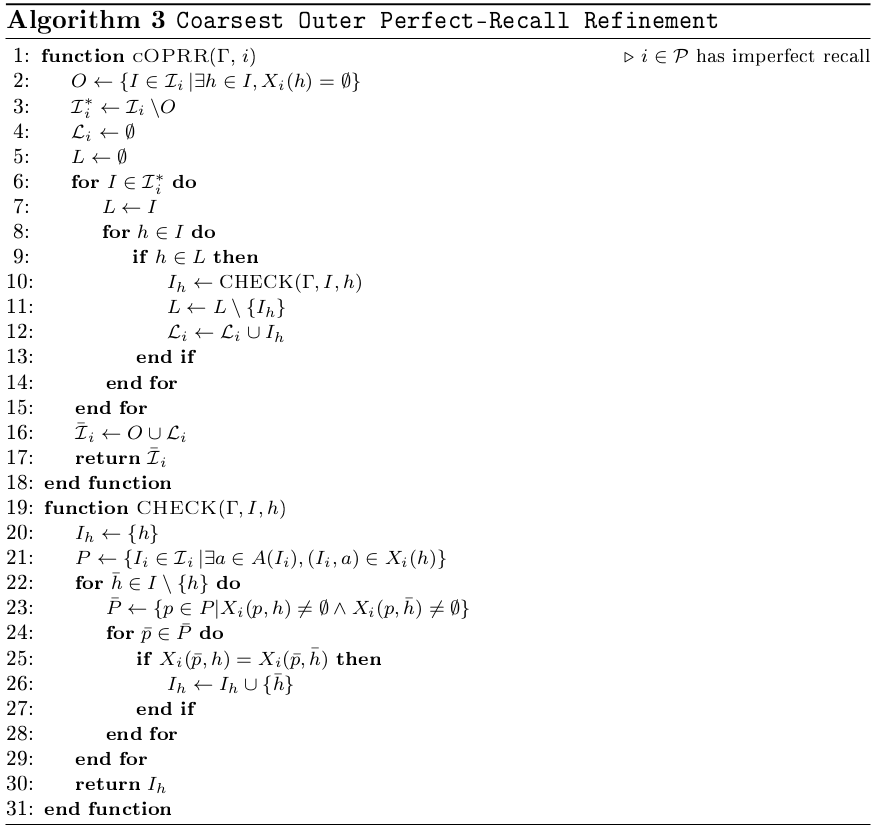
\includegraphics[width=0.7\textwidth]{coarsest}
\end{frame}

\begin{frame}
\centering
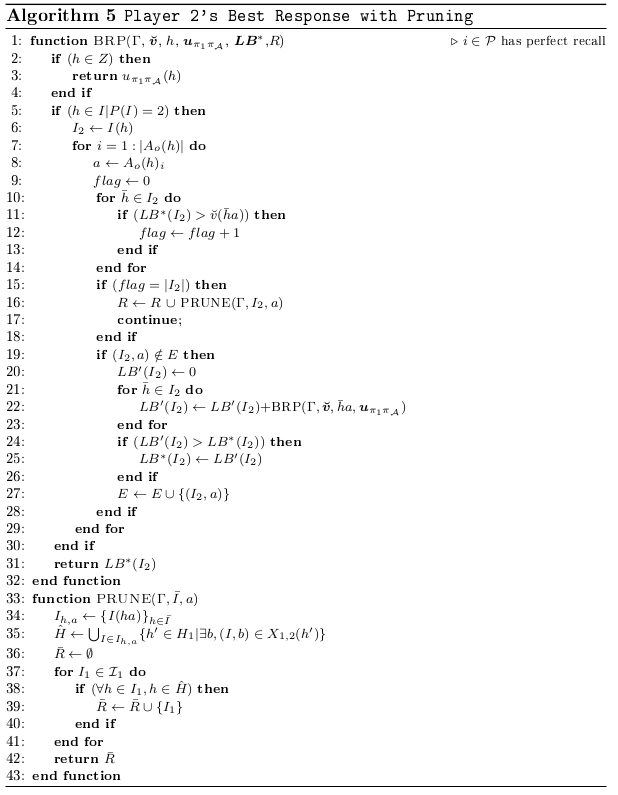
\includegraphics[width=0.55\textwidth]{br}
\end{frame}

\end{document}

